\chapter{Experiments}

\section{Generating the obstacle forest (Poisson processes)}

In order to generate the obstacle field for the experiments, which is to
resemble a forest, a spatial process called a \textit{Poisson process} is
employed. Poisson processes are used to model random configurations of points in
space'~\cite{kroeseSpatialProcessGeneration}, and hence are suitable for
generating a simulated forest. For the experiments below, a forest will be the
realization of a spatial Poisson process on \(\R^2\).

A few key parameters of the Poisson process has to be set for use in the
experiments below. Firstly, \(\lambda\) is the intensity of the spatial process.
For these experiments, the intensity will be held constant, and the process is
therefore homogeneous, as it does not vary with the position in space. One
interesting configuration could be to vary the intensity as the radius from
origo, and hence the difficulty in traversing the terrain would increase with
the distance travelled. However, the constant intensity setting was chosen to
keep things simple and uniform.

The algorithm for realizing a random Poisson measure~(\ref{def:Poisson-def}) is
taken from~\cite[Definition 1.1.1,p~34]{kroeseSpatialProcessGeneration}.

\begin{definition}[Generating a Poisson random measure]
  \label{def:Poisson-def}
  \begin{enumerate}
  \item Generate a Poisson random variable \(N ~ Poi(\mu(E))\).
  \item Draw \(X_1,X_2,\ldots,X_N ~ g\), where \(g(x) \lambda(x)/ \mu(E)\).
  \end{enumerate}
\end{definition}
where \(E\) is the set over which the points should be generated, and the
\textit{pdf} \(g(x_1, x_2) = \lambda(x)/\mu(E)\). Finally, \(\mu(E)\) is defined
as
\[
  \mu(E) = \int_{E} \lambda(x) dx.
\]

For the experiments the set \(E\) will be a square defined as
\[
  E = [-\alpha, \alpha]^2
\]
the density of the generated forest \(\lambda\) will be set to
\[
  \lambda = 0.09
\]
of which the resultant forest on a \(20 \times 20\) grid can be seen in
figure~(\ref{fig:poisson009})

\begin{figure}
  \centering
  \begin{minipage}[b]{0.4\textwidth}
    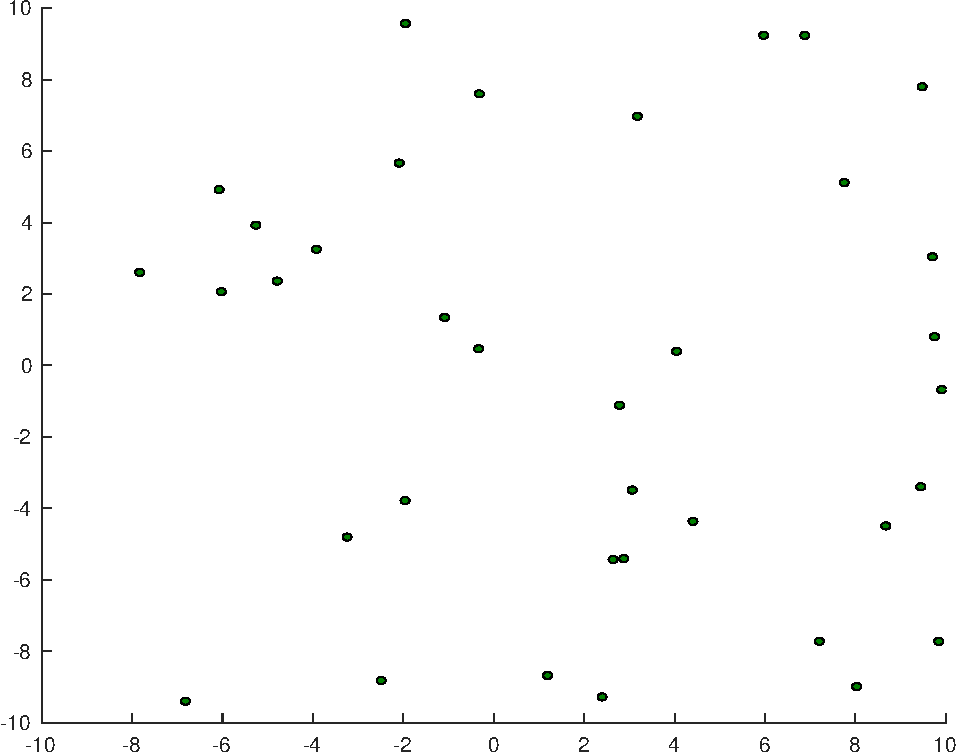
\includegraphics[width=\textwidth]{figures/experiments/poisson009}
    \caption{The resultant forest generated by a spatial Poisson process with
      intensity \(\lambda = 0.09\)}
    \label{fig:poisson009}
  \end{minipage}
  \begin{minipage}[b]{0.4\textwidth}
    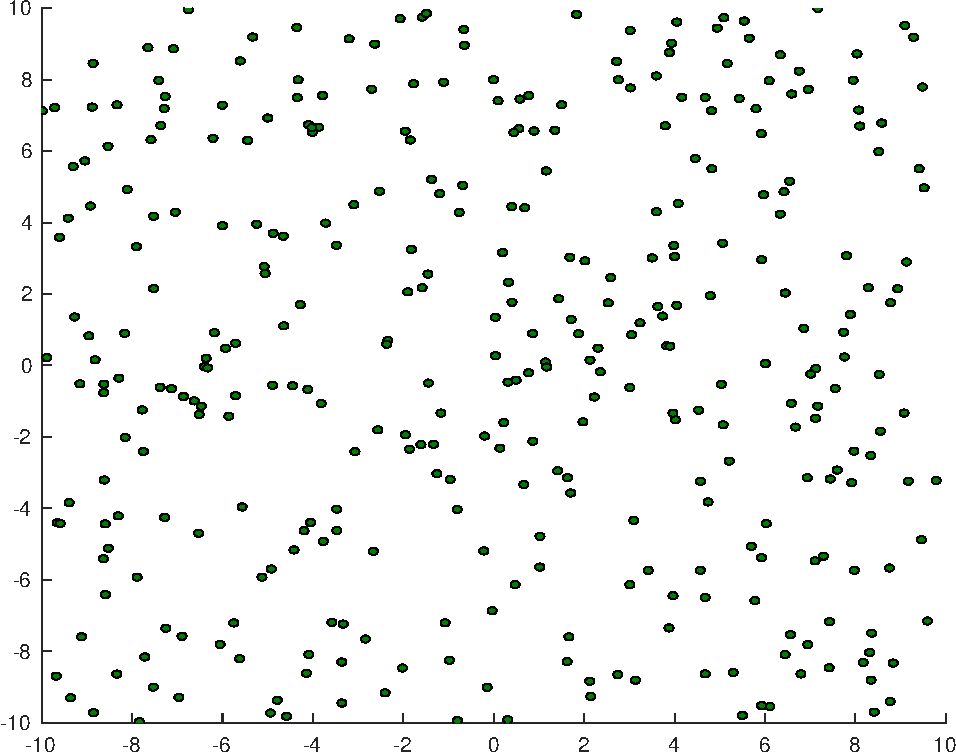
\includegraphics[width=\textwidth]{figures/experiments/poisson09}
    \caption{The resultant forest generated by a spatial Poisson process with
      intensity \(\lambda = 0.9\)}
    \label{fig:poisson09}
  \end{minipage}
\end{figure}

\section{Deciding upon the size of the vehicle and the obstacles}

The funnels generated thus far is created from a point model of the vehicle, and
it's dynamics. In the case that the grid that the simulations are run on are set
to have an increment of a meter, then the funnels from the basic set are given a
velocity of \([v(t)] = \si{m.s^{-1}}\), \([\theta] = \si{\radian\per\second}\),
and \([\dot{\theta}] = \si{\radian\per\second\per\second}\), where \([\cdot]\)
is the unit operator. The size of the vehicle is arbitrary, and can be chosen
freely, but if it is imagined as a radio controlled car, with a speed of
\(10\si{m.s^{-1}}\), then a size of \(30 \times 20 \si{\centi\metre} \) keeps
everything within the realm of a normal radio controlled car and its
capabilities. The mass is not relevant for our first order dynamics, but still
the vehicle is assigned a mass of \(1 \si{\kilo}\), so that the translation of
the model dynamics is not irrelevant.

\subsection{Expanding the size of the funnel by the size of the simulated
  vehicle}

The size of the vehicle in the original model a single point, and as such, not
accounted for in the funnel before running simulations. Therefore the funnels
have to be expanded in order for them to accomodate the necessary robustness
guarantees that are expected. However, the size of the vehicle only affects the
size of the funnel ellipsis projected down into the xy-plane. Therefore first
getting the projected size of the funnel where \(P \colon \R^4 \rightarrow
\R^2\) is a projection map with a projection matrix
\[
  P =
  \begin{bmatrix}
    I & \mathbf{0} \\
  \end{bmatrix}
\]
such that for the projected ellipsoid
\[
  \mathcal{E}_{p} = \set{\bar{x} \in \R^{2} \mid {\bar{x}}^{T}S_{k}^{(p)}\bar{x}
    \leq 1}
\]
and
\[
  S_{k}^{(p)} = \left( PS_{k}^{-1}P^T \right)^{-1}
\]
and \(\mathcal{E}_{p}\) is the projected set of the ellipsoid projected down
into the xy-plane~\cite{majumdarFunnelLibrariesRealtime2017}. In general an
ellipse centered at the origin is a linear transformation of the unit
circle~\cite{lay2005linear}. Exploiting this fact, expanding the radius of the
circle to encompass the vehicle model. Also taking into account that the matrix
\(S_{k}\) is \textit{Positive semidefinite}, and hence can be cholezky
factorized~\cite{lay2005linear}. The expanded ellipsis (which now contains all
the possible states of the vehicle model) is:

\begin{align*}
  S_{k}^{\mathcal{P}} &= R^{T}R \\
  \mathcal{C} &= \set{y \in \R^2 \mid y^{T}y \leq 1 + r_{vehicle}} \\
  S_{k}^{p'} &= R^{-1}y \\
\end{align*}

where \(S_{k}^{'}\) is the ellipsoid which contains the volume of the vehicle
for all verfied states in the funnel.

\subsection{Terrors of errors}

The funnel compuatations error out if too much uncertainty is added. In this
case that is velocity higher than two (which to be fair is a bit). Also, the
length of the funnels error out, meaning that funnels longer than approximately
.3 seconds, which is what they are now, will error out. Had there
been more time this should probably be resolved. A guess is that increasing the
sampling frequency, and/or increasing the initial size of the \(\rho\) guess
would help.